\capitulo{4}{Técnicas y herramientas}

En este apartado describiremos las técnicas y herramientas
que hemos usado para la realización de este proyecto.

\section{Técnicas utilizadas para el funcionamiento de la página WEB}

\subsection{\textit{Solidity}}

\textit{Solidity}\cite{solidity}\cite{solidity1}\cite{solidity2} es un lenguaje de programación de alto nivel, está diseñado para crear y desarrollar contratos inteligentes que se ejecuten en la \textit{Machine Virtual Ethereum}(EVM). La síntesis es similar a \textit{Javascript}.

\begin{wrapfigure}{r}{0.4\linewidth}
    \centering
    
\includegraphics[width=0.20\textwidth, scale=0.5]{solidity}
    \caption{Logo \textit{Solidity}}
\end{wrapfigure}

Al estar diseñado para el desarrollo de Contratos Inteligentes, se dice que es algo limitado en el uso, aunque este lenguaje también está considera en el ámbito de la programación como muy poderoso.

\textit{Solidity} funciona con la creación de contratos ``Smart Contracts'' lo cual ayuda a que muchas partes de un negocio funcionen correctamente por si mismas y se pueda llevar un mejor control de registro de las acciones actividades mencionadas anteriormente.\\

\subsection{\textit{HTML} y \textit{CSS}}

\textit{HTML}\cite{html},\textbf{HyperText Markup Language} ``Lenguaje de Marcas de Hipertexto'' es un lenguaje de marcado que se utiliza para el desarrollo de páginas páginas web.

Al contrario de lo que mucha gente piensa, no te incluye el diseño gráfico de la página web, esta herramienta solo sirve para decir cómo va organizado el contenido de nuestra página web. Esto se consigue a través de las llamadas marcas de hipertexto ``más común mente llamas etiquetas'' o mediante su nombre en inglés como ``tags''.

\begin{wrapfigure}{r}{0.4\linewidth}
    \centering
    
\includegraphics[width=0.20\textwidth]{html}
    \caption{Logo \textit{HTML}}
\end{wrapfigure}

Actualmente se puede decir que HTML es el lenguaje estándar que se ha
impuesto en la visualización de páginas web, ya que es el que todos los
navegadores del momento han adoptado.

En el proyecto empleamos \textit{HTML} para la creacción de la parte \textit{front} de la aplicación \textit{web}.\\\\

\textit{CSS}\cite{css} o Cascading Style Sheets (Hojas de estilo en cascada)se puede un considerar una buena elección porque permite implementar un diseño gráfico para definir y realizar la presentación de una página o documento estructurado escrito en un lenguaje de marcado\cite{marcado}\footnote{Lenguaje de marcado: consiste en codificar un documento el cual incorpora etiquetas que contienen información adicional que nos informa de la estructura del texto o de su presentación en cada momento}.

CSS permite poder ser usado en la presentación de los documentos HTML. Con este lenguaje podemos elegir una amplia variedad de opciones de presentación véase: colores, tamaño de letra y posición de imágenes.

\begin{wrapfigure}{l}{0.4\linewidth}
    \centering
    
\includegraphics[width=0.20\textwidth]{css}
    \caption{Logo \textit{CSS}}
\end{wrapfigure}

El objetivo principal de CSS es intentar diferenciar o separar la estructura HTML de la presentación. La web sería lo que se encuentra en la parte inferior, el contenido, y el CSS se podría decir que es lo que hace que se vea el contenido, permitiendo al programador decidir el programador la forma que se vea.\\

Para la elaboración de nuestros CSS nos hemos ayudado de la pagina w3school: \url{https://www.w3schools.com/css/default.asp}

\subsection{\textit{PHP}}

PHP\cite{php1} es un lenguaje es de código abierto que está preparado, entre otras cosas, para el desarrollo web y puede ser incrustado en HTML. Esta fue una de las principales razones para utilizar este lenguaje.

\begin{wrapfigure}{r}{0.4\linewidth}
    \centering
    
\includegraphics[width=0.20\textwidth]{php}
    \caption{Logo \textit{PHP}}
\end{wrapfigure}

Hypertext Pre-processor PHP\cite{php}, es un lenguaje de programación y posterior maquetado, ya que es posible implementar diversas instrucciones que consigan obtener resultados, y conseguir la comunicación con el servidor de datos para la web.\\

Uno de los grandes motivos por los que se ha utilizado PHP, aparte de por su uso durante el proceso del grado, es por ser una multi-plataforma gratuita. Con esta razón daría igual el sistema operativo con el que estuviéramos trabajando.



\section{Técnicas utilizadas para el la conexión entre la web y nuestro Smart Contract}

\subsection{\textit{Truffle}}

\textit{Truffle}\cite{truffle} es un \textit{framework} de desarrollo de \textit{Ethereum} que facilita la labor a la hora de desarrollar, testar y desplegar los \textit{smart contracts}.

Un \textit{Framework}:  conjunto estandarizado de conceptos, prácticas y criterios para enfocar un tipo de problemática particular que sirve como referencia, para enfrentar y resolver nuevos problemas de índole similar.

\textit{Truffle} nos ofrece la posibilidad de:

\begin{itemize}
	\item Compilación, enlace y despliegue de Smart contracts desde el propio \textit{framework}.
	\item Depuración y \textit{testing} automatizado de contratos.
	\item \textit{Framework} con \textit{scripts} de despliegue y migraciones en redes públicas y privadas.
	\item Acceso a cientos de paquetes externos y gestión con \textit{EthPM \& NPM}.
	\item Aplicación de una consola interactiva para comunicación directa con los contratos.
	\item Interacción con contratos mediante \textit{scripts} externos.
\end{itemize}
 
Una capacidad de \textit{Truffle} es desplegar nuestros \textit{Smart contracts} de manera muy sencilla a distintos entornos. Los cuales se podrán modificar desde el \textit{truffle-config.js}. Hablaremos de su intalación en el apartado de los anexos. 

\subsection{\textit{Remix}}

\textit{Remix}\cite{remix} es un IDE basado en navegador web que le permite escribir contratos inteligentes de Solidity para luego implementar y ejecutar el contrato inteligente.

\begin{wrapfigure}{r}{0.4\linewidth}
    \centering
    
\includegraphics[width=0.20\textwidth]{remix}
    \caption{Logo \textit{Remix}}
\end{wrapfigure}

La página es mediante Internet y es: \url{https://remix.ethereum.org/#optimize=false&version=soljson-v0.4.24+commit.e67f0147.js} \textit{Remix} te dejará seleccionar el tipo de versión para la compilación y desde dónde realizaremos la ejecución de nuestro \textit{smart contract}, que será una red local como es \textit{Ganache} o será una red exterior.

El objetivo de usar este programa es conseguir lo siguiente:

\begin{itemize}
	\item Crear los contratos inteligentes y depurar la ejecución.
	\item Poder saber el estado y las propiedades de los \textit{smart contract} que se han creado anteriormente.
	\item Reducir errores de codificación y poder aplicar mejoras, con un análisis del código.
\end{itemize}

Remix es normalmente utilizado para pequeños contratos, ya que no necesita una instalación y lo podremos usar tanto \textit{on-line} como \textit{off-line}, pudiendo descargar un archivo y, a la hora de ejecutar, poder usar el ``index.html''

Para los programas más grandes tendremos la opción de utilizar node.js (del cual hablaremos a continuación) o Docker entre otros.

\subsection{\textit{Node.js}}

Node.js\cite{node}\cite{node1} es un entorno en tiempo de ejecución multiplataforma de código abierto.

Esta concebido como entorno de ejecución de JavaScript y esta orientado a eventos asíncronos, el objetivo es construir aplicaciones en las redes escalables. 

Por cada conexión callback este sera ejecutado, pero si no tiene trabajo que realizar node.js estará en modo hibernación, con node.js no tenemos que preocuparnos por si el proceso se bloquea, node.js siempre realiza I/O directamente esta es la razón por la que nunca se bloquea. Esta es una de las grandes razones por es se desarrolla en sistemas escalables.

%%  \cite{node1}
%%\begin{wrapfigure}{r}{0.4\linewidth}
  %%  \centering
   %%   
\includegraphics[width=0.20\textwidth]{node}
  %%    \caption{Logo \textit{Node.js}}
%%  \end{wrapfigure}

\subsection{\textit{Metamask}}

MetaMask\cite{metamask} es un complemento de navegador que permite a los usuarios realizar transacciones de Ethereum a través de sitios web regulares.

MetaMask\cite{metamask1} es una herramienta \textit{plugin} que sirve como puente entre las \textit{dapps} y el navegador Chrome. Al usar esto nunca se compromete la seguridad, siendo posible el uso de varias cuentas y teniendo la suerte de no tener que llegar a usar un nodo Ethereum de forma completa.

La aplicación fue desarrollada con la intención de acercar la tecnología blockchain al usuario a través de una serie de DApps\footnote{\textit{``decentralized application''} o aplicaciones descentralizadas}, las cuales funcionan como una extensión del navegador. Con ellas tenemos las opciones de:
\begin{itemize}
	\item Acceder a servicios
	\item Firmar transacciones blockchain
	\item Administrar tokens
	\item Administrar varios monederos
\end{itemize}

Todos estos puntos anteriores se intentan conseguir en una interfaz amigable y segura. 

\begin{figure}[h]
	\centering
  
\includegraphics[width=0.7\textwidth]{metamask}
  \caption{Metamask}
\end{figure}

La idea es integrar todos los servicios, incluyendo aquellos de Ethereum, en el navegador.

Una de las grandes preguntas que nos surgen al usar Metamask, es si es segura, de acuerdo con los investigado y leído hasta la fecha en diferentes paginas web no ha sufrido ningún daño, y tampoco se tiene constancia de que se haya realizado robos de criptomonedas por ningún hacker.

Metamask utiliza un sistema de seguirdad al cual se le llama HD, este consigue mantener todas las claves locales cifradas y gracias a ello se cumple el objetivo que las Dapps no tengan la posiblidad de acceder a ellas.

El sistema sistema de seguridad que tiene es conocido como ``palabras semillas'', las cuales tienen un orden concreto y sirven para recuperar la cuenta en el caso de que esta fuera robada.
 
Algo contra lo que intenta luchar Metamask es la suplantación de identidad, phishing, también conocido como billetera on-line. Metamask lleva tiempo intentando combatir este problema. 
 
\subsection{\textit{Ganache}}

\textit{Ganache}\cite{ganache} sirve para poder desarrollar aplicaciones en Ethereum y se realiza sobre una red local para realizar las pruebas. 

Las pruebas serán como si estuvieramos trabajando sobre la red Ethereum de verdad, pero con la ventaja de que requiere tantos recursos y el desarrollo es más rápido. 

Este programa es un simulador de la \textit{blockchain} para Ehtereum en el que podremos desplegar contratos, ejecutar nuestros \textit{tests}, ejecutar comandos o inspeccionar el estado de la red.

\begin{figure}[h!]
  \centering
  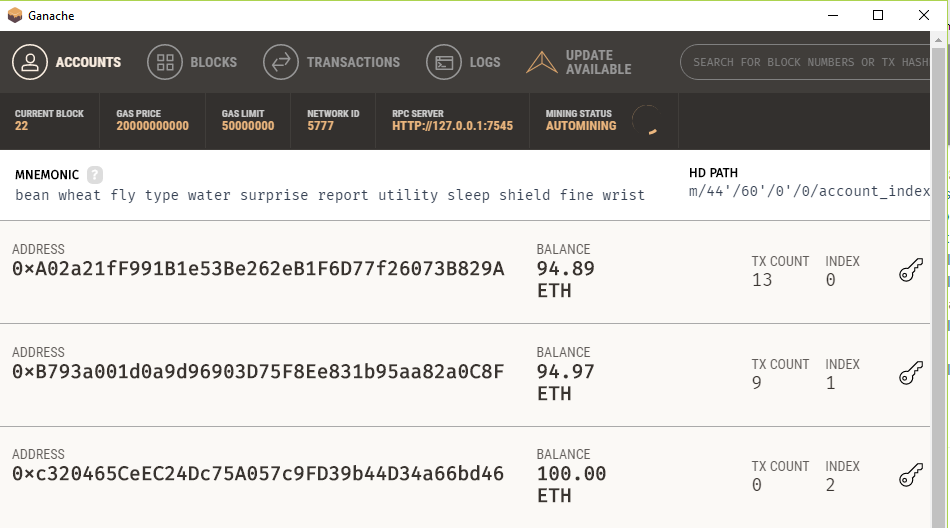
\includegraphics[width=0.5\textwidth]{ganache}
  \caption{Ganache}
\end{figure}
\section{Herramientas utilizadas para el funcionamiento de la página web, funcionando con base de datos}

\subsection{\textit{Visual Studio Code}}

Visual Studio Code\cite{VisualStudio} es un editor de texto con el cual hemos realizado gran parte de nuestro proyecto, tanto para el HTML como para la realización de los contratos una vez pasados por la plataforma Remix así como para realizar los procesos correspondientes para coger formato de nuestro contrato con JSON.

Nos decantamos por usar Visual Stuido\cite{VS-code} code ya que la edición de código no está limitada para los programas C\# o Visual Basic, sino que acepta mas programas como php, html, solidity \ldots que son los principales percusores de nuestro trabajo final. 

Otra parte positiva de este editor es la función ``IntelliSense'', la cual permite al usuario de este programa poder ahorrar tiempo al escribir instrucciones, ya que tiene una función de auto-completar con el propio editor, esto logra hacer que el trabajo sea mas productivo, acortar la escritura y no cometer errores por la sintaxis.

\subsection{\textit{XAMPP}}

La siguiente herramienta de la que hablaremos será de la creación de la base de datos, en este caso hemos querido usar XAMPP\cite{xampp}(X\footnote{X: hace referencia a que sirve para cualquiera de los diferentes sistemas operativos} Apache, MySQL, PHP, Perl.)

En el apartado 5, ``Aspectos relevantes del desarrollo del proyecto'' y en los anexos hablaremos mas específicamente sobre este programa. Explicaremos cómo realizar la instalación y el uso que le damos en nuestra aplicación. Por el momento daremos una breve introducción de por qué hemos seleccionado esta en vez de otro programa similar.

Una vez lo tengamos instalado, podremos realizar crear, editar, consultar y gestionar bases de datos en MySQL de una manera eficaz y limpia.

Al usar este programa, hemos retomado cómo poder administrar las bases de datos y su acceso a una base de datos desde PHP, así como realizar diferentes SELECT y sacar el resultado por página web.

\section{Control de versiones y documentación}

En el siguiente apartado veremos las herramientas que utilizamos para el control de las versiones y la herramienta empleada para el desarrollar del documento de este proyecto.

\subsection{\textit{Látex}}

\textit{LaTeX}\cite{latex} es un sistema de preparación de documentos. Con este programa podemos cartas, tesis, presentaciones y cualquier tipo de documento que quisieras imprimir en papel o mostrar en pantalla. 

La principal opción por la que usamos \textit{LaTex} es porque tiene una mejor calidad de tipografía en comparación con los editores convencionales.

Para el proyecto usamos \textit{TexMaker} en la versión para \textit{Windows}.

\subsection{\textit{GitLab y GitHub}}

\textit{Gitlab}\cite{gitlab} o \textit{GitHub}\cite{github} son servicios web para el control de versiones y desarrollo de software colaborativo basado en \textit{Git}.

Utilizamos este programa para mostrar el proyecto finalizado. El repositorio se tendrá acceso en el siguiente repositorio \cite{repositorio},pero este repositorio es privado por lo cual hemos creado uno público en \textit{gitHub} y se podrá observar la información en la pagina \cite{repositorio1}.

%\begin{figure}[h]
%    \centering
%    \includegraphics[width=0.5\textwidth]{gitLab}
%	\caption{{Logotipo del programa \textit{GitLab}}}
%\end{figure}
%\begin{wrapfigure}{r}{0.4\linewidth}
%    \centering
%    \includegraphics[width=0.20\textwidth]{gitLab}
%    \caption{Logotipo del programa \textit{GitLab}}
%\end{wrapfigure}

